\documentclass[preview,border=5pt]{standalone}
\usepackage{teaching}
\begin{document}

\centering

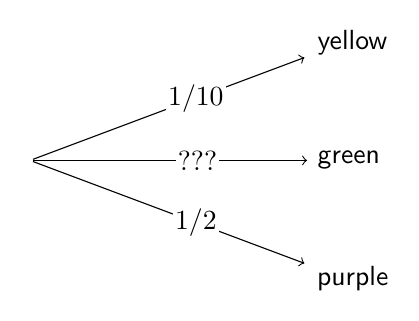
\begin{tikzpicture}[yscale=1,xscale=1,scale=2,inner sep=0.3mm, label distance=1.5mm]

\node(o) at (-2,0) {};
\node(h) at (0,0.75) {\;\;\textsf{yellow}};
\node(t) at (0,0) {\;\textsf{green}};
\node(g) at (0,-0.75) {\;\;\textsf{purple}};
\draw[->] (o) -- (h) node [pos=0.6, fill=white] {$1/10$};
\draw[->] (o) -- (t) node [pos=0.6, fill=white] {$???$};
\draw[->] (o) -- (g) node [pos=0.6, fill=white] {$1/2$};

%\node(a1) at (1.5,1.75) {$1$};
%\node(a2) at (1.5,1.45) {$2$};
%\node(a3) at (1.5,1.15) {$3$};
%\node(a4) at (1.5,0.85) {$4$};
%\node(a5) at (1.5,0.55) {$5$};
%\node(a6) at (1.5,0.25) {$6$};
%
%\node(b1) at (1.5,-1.75) {$6$};
%\node(b2) at (1.5,-1.45) {$5$};
%\node(b3) at (1.5,-1.15) {$4$};
%\node(b4) at (1.5,-0.85) {$3$};
%\node(b5) at (1.5,-0.55) {$2$};
%\node(b6) at (1.5,-0.25) {$1$};
%
%\node(h1) at (1.9,1.74) {$(H1)$};
%\node(h2) at (1.9,1.44) {$(H2)$};
%\node(h3) at (1.9,1.14) {$(H3)$};
%\node(h4) at (1.9,0.84) {$(H4)$};
%\node(h5) at (1.9,0.54) {$(H5)$};
%\node(h6) at (1.9,0.24) {$(H6)$};
%
%\node(t1) at (1.9,-1.76) {$(T6)$};
%\node(t2) at (1.9,-1.46) {$(T5)$};
%\node(t3) at (1.9,-1.16) {$(T4)$};
%\node(t4) at (1.9,-0.86) {$(T3)$};
%\node(t5) at (1.9,-0.56) {$(T2)$};
%\node(t6) at (1.9,-0.26) {$(T1)$};
%
%
%\draw[->] (h) -- (a1);
%\draw[->] (h) -- (a2);
%\draw[->] (h) -- (a3);
%\draw[->] (h) -- (a4);
%\draw[->] (h) -- (a5);
%\draw[->] (h) -- (a6);
%
%\draw[->] (t) -- (b1);
%\draw[->] (t) -- (b2);
%\draw[->] (t) -- (b3);
%\draw[->] (t) -- (b4);
%\draw[->] (t) -- (b5);
%\draw[->] (t) -- (b6);

\end{tikzpicture}

\end{document}